\chapter{Deep Learning}

\section{Lesson Outline}
Deep learning has a surprisingly long history but has become popular only relatively recently. In this lesson, we will learn:

\begin{itemize}
    \item How experts think about Deep Learning
This gives us a framework to understand when we should be using Deep Learning.

    \item The differences between Artificial Intelligence, Machine Learning, and Deep Learning
    \item The origins and history of Deep Learning
    \item Tools for using Deep Learning
    \item Applications of Deep Learning
\end{itemize}
This lesson will provide you with a framework and context necessary to make decisions about where and when to apply deep learning.

\section{How Do Experts Think About Deep Learning?}
Whether or not deep learning is the path to artificial general intelligence, experts all understand the power of Deep Learning to accomplish a variety of tasks. Practitioners in the field recognize some shortcomings in Deep Learning, but its power on computer vision and Natural Language processing tasks is undeniable.

Drawbacks of deep learning:
\begin{itemize}
    \item lack of causality
    \item lack of interpretability 
    \item need to double-check predictions 
\end{itemize}

\section{AI, ML, and Deep Learning}
As we can see, Artificial Intelligence is the overarching field and includes algorithms like Local Search and Logic Programming. Machine Learning \textit{is a part of} Artificial Intelligence and includes models like Logistic Regression and Decision Trees. Deep Learning \textit{is a subfield of} Machine Learning that consists of various neural network models.

  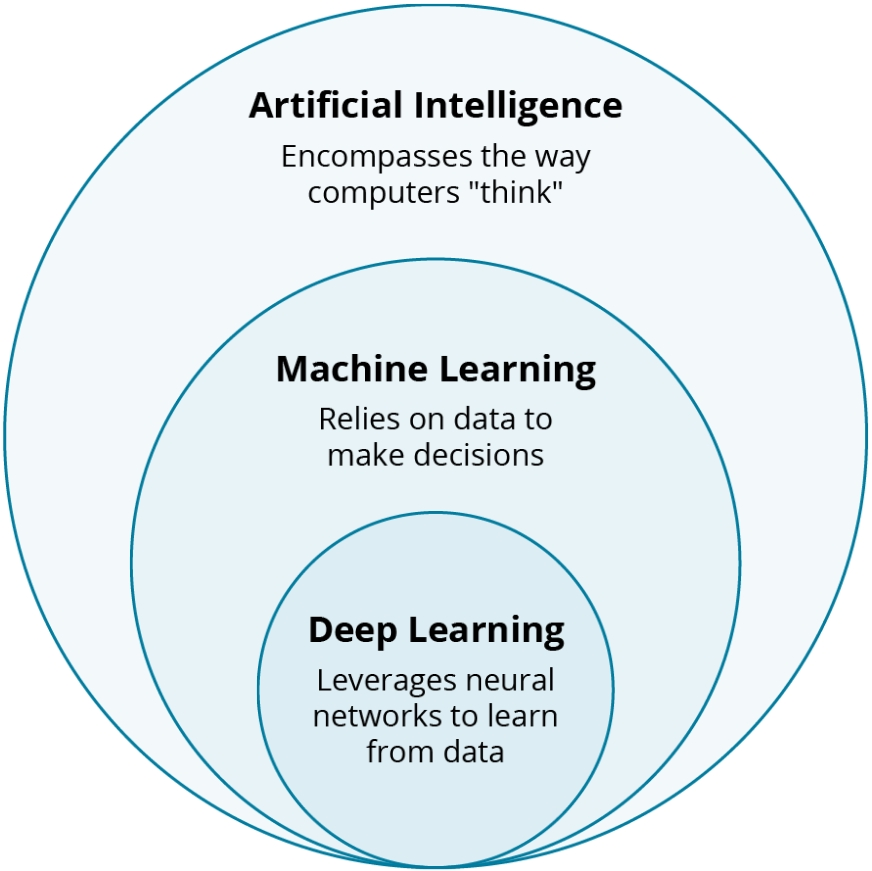
\includegraphics[width=1\linewidth]{img//intro/aimldl.jpeg}

\section{Tools for Deep Learning}
We begin with a problem statement, then move to development (where code gets written). Next, we begin training, where our model learns our data. After training, we deploy, which is when our model goes out into the world for use. A lot of other people do front-end work at this stage. Then we go to monitoring. For our purposes, we'll focus on the \textbf{development} and \textbf{training} of models.

\subsection{Development tools}

\begin{itemize}
    \item Integrated Development Environment

\begin{itemize}
        \item Code Editor
        \item Interpreter/Compiler
\end{itemize}

    \item Jupyter Notebooks
Note: Each cell is executed on its own, and it works well for environments to prototype or present code. However, there are limitations:

\begin{itemize}
        \item Editing can make you lose state
        \item Code deployed production should be in .py rather than notebooks
\end{itemize}

\end{itemize}

\subsection{Deep Learning Frameworks}

\begin{itemize}
    \item PyTorch (aka Torch)
    \item TensorFlow/Keras
    \item JAX
\end{itemize}

\subsection{Training Tools}

\begin{itemize}
    \item Experiment management like TensorBoard or Weights and Biases
    \begin{itemize}
    \item Observe accuracy and loss at training time
    \end{itemize}
    \item Model versioning like DVC, Neptune, and Pachyderm: Model versioning tools are great for looking at historical trends and comparing different versions of the model against one another.
\begin{itemize}
        \item Remedy issues within the model across different versions of the model
        \item DVC is very similar to Git
\end{itemize}

\end{itemize}

\section{When To Use Deep Learning}
\href{https://www.youtube.com/watch?v=nYFmdOMXoz0&t=57s&ab_channel=Udacity}{Youtube}

\subsection{No Free Lunch Theorem}
There is no single algorithm that performs better across all possible functions. \textbf{There is no one algorithm to rule them all}.

Skepticists: This is a theoretical result over the infinite space of possible functions and that in reality, there are algorithms that perform better on the types of problems that we're interested in. 

We should consider deep learning when we're playing to its strengths:

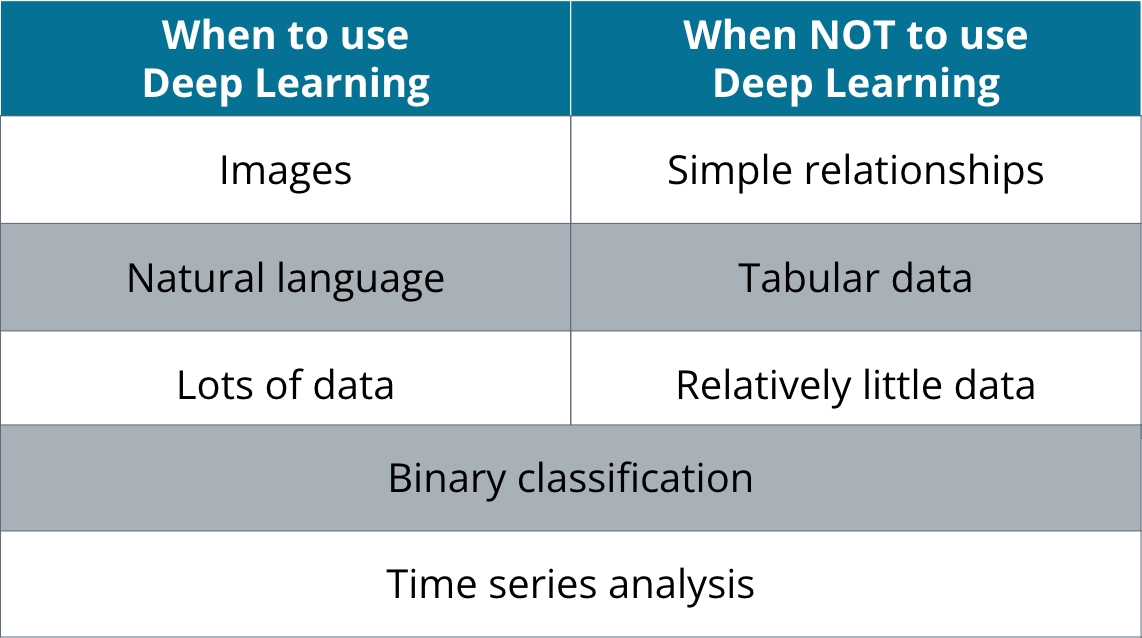
\includegraphics[width=1\linewidth]{img//intro/screen-shot-2022-06-27-at-11.03.33-am.jpeg}
\captionof{figure}{When and When Not to Use Deep Learning}

Deep Learning is a powerful tool, but it's not the only one. In general, the way to choose whether or not to use Deep Learning depends on your task, what kind of data you have, and how complex the relationships in the data are.

Scenarios in which to use Deep Learning include but are not limited to:

\begin{itemize}
    \item \textbf{Tasks}

\begin{itemize}
        \item Binary classification:

    \begin{itemize}
            \item Deep Learning
            \item Logistic Regression
            \item Decision Trees
            \item Support Vector Machines
    \end{itemize}

        \item Multi-class classification:

    \begin{itemize}
            \item Deep Learning
            \item Decision Trees
            \item Support Vector Machines
    \end{itemize}

        \item Regression:

    \begin{itemize}
            \item Deep Learning
            \item Linear Regression
            \item some Decision Trees
    \end{itemize}

\end{itemize}

    \item \textbf{Data:}

\begin{itemize}
        \item Images:
Deep Learning

        \item Text:

    \begin{itemize}
            \item Deep Learning
            \item Statistical Methods
    \end{itemize}

        \item Tabular Data:
Decision Trees

\end{itemize}

    \item \textbf{Data Relationships}:

\begin{itemize}
        \item Simple:

    \begin{itemize}
            \item Linear Regression
            \item Logistic Regression
            \item Decision Trees
    \end{itemize}

        \item Complex:

    \begin{itemize}
            \item Deep Learning
            \item Decision Trees
    \end{itemize}

\end{itemize}

\end{itemize}

\subsection{Additional Resources}

If you want to learn more about when each machine learning method is appropriate, we recommend\href{https://mitsloan.mit.edu/ideas-made-to-matter/machine-learning-explained}{\textbf{ this article from MIT's Sloan school}}\newline

Model interpretability is an important constraint on our model choice, and unfortunately makes neural networks less-than ideal for our problem. That leaves logistic regression and decision trees as interpretable models we can use for binary classification problems in this scenario.

\section{(Optional) Computer Vision Demo: TinyYOLOv2}

\subsection{Computer Vision Object Detection Model}

Deep learning is used for myriad applications, from sentiment analysis (Natural Language Processing) and image recognition (Computer Vision) to the generation of text and images (Multimodal).

\href{https://arxiv.org/abs/1506.02640}{\textbf{You Only Look Once, or YOLO}}, is an \href{https://en.wikipedia.org/wiki/Object_detection}{\textbf{object recognition}} model still very effective today, years after its release. The model is based on a \href{https://stanford.edu/~shervine/teaching/cs-230/cheatsheet-convolutional-neural-networks}{\textbf{Convolutional Neural Network}} architecture, i.e., a specialized deep learning architecture primarily used in Computer Vision.

YOLO uses anchor boxes to predict the coordinates of the bounding boxes around objects. It also applies non-maximum suppression to remove duplicate detections and refine the bounding box locations. This model is known for its speed and accuracy, making it a popular choice for real-time object detection applications, such as self-driving cars, surveillance systems, and robotics.

At a high level, YOLO and other convolutional neural networks take images of 3-dimensional tensors -- you can think of a Rubik's cube as a 3 x 3 x 3 tensor -- that uses a mathematical operation called convolution to generate representations of different properties of an image. These properties are passed on to further layers that identify other properties of an image and, eventually, output a prediction about the image.

\subsection{TinyYOLOv2 - YOLO Lightweight Model}

Carnegie Mellon University has a TinyYOLOv2 implementation available \href{https://www.cs.cmu.edu/~dst/FaceDemo/index.html}{\textbf{for experimentation}} that explores pre-loaded images and allows new images to be uploaded. TinyYOLO is much faster but less accurate than the standard YOLO model.

The TinyYOLOv2 model is a real-time neural network that detects 20 different classes and comprises nine convolutional layers and six max-pooling layers. This model is lightweight and designed to be computationally efficient, making it a good choice for applications with limited computing resources, such as live webcams, mobile devices, or embedded systems.

\section{Optional) Image Generation Demo: DALL·E Mini}

\href{https://openai.com/research/dall-e}{\textbf{DALL-E}} is a project from OpenAI designed to generate images from text. There are many other systems now for generating these images, such as \href{https://www.midjourney.com/}{\textbf{Midjourney}} and \href{https://huggingface.co/spaces/stabilityai/stable-diffusion}{\textbf{Stable Diffusion}}. These image generation models are a class of physics-inspired \href{https://en.wikipedia.org/wiki/Diffusion_model}{\textbf{Diffusion Model}}.

\href{https://github.com/borisdayma/dalle-mini}{\textbf{DALL-E mini}} is a smaller version of the DALL·E model designed to run on consumer-grade equipment but still offers excellent performance!

\begin{quote}
If you are interested in learning more about DALL·E Mini dataset, architecture, and model training, you can read this article by the authors: \href{https://wandb.ai/dalle-mini/dalle-mini/reports/DALL-E-mini--Vmlldzo4NjIxODA}{\textbf{DALL·E Mini Explained}}

\end{quote}

\subsection{Exercise}

In this exercise, you can experiment with creating images from texts using the DALL-E Mini model in two ways:

\begin{enumerate}
    \item \href{https://huggingface.co/spaces/dalle-mini/dalle-mini}{\textbf{No-code DALL·E Mini demo}} by \href{https://www.craiyon.com/}{\textbf{craiyon.com}} on HuggingFace Space
    \item Run DALL·E Mini inference pipeline on Jupyter Notebook \href{https://github.com/borisdayma/dalle-mini/blob/main/tools/inference/inference_pipeline.ipynb}{\textbf{[GitHub link]}} \href{https://colab.research.google.com/github/borisdayma/dalle-mini/blob/main/tools/inference/inference_pipeline.ipynb}{\textbf{[Google Colab link]}}
\end{enumerate}

\textit{\textbf{Notes on DALL·E Mini Inference Pipeline Notebook:}}

\begin{enumerate}
    \item Before you run the Jupyter Notebook, you need to get an API key from \href{https://wandb.ai/}{\textbf{wandb.ai}}.
You can create a new account and find the API key here: \href{https://wandb.ai/authorize}{\textbf{https://wandb.ai/authorize}}.

    \item The notebook requires \verb|jax| and \verb|jaxlib| libraries v0.3.25.
After you run the first cell to pip install \verb|dalle-mini| and \verb|vggan-jax|, create a new cell, and install \verb|jax| and \verb|jaxlib| v0.3.25

\end{enumerate}

\begin{quote}
!pip install jax==0.3.25

!pip install jaxlib==0.3.25

\end{quote}

Right-click and save DALL·E Mini Inference Pipeline Jupyter Notebook with the correct jax library \href{https://video.udacity-data.com/topher/2023/March/641ba138_dalle_mini_inference_pipeline/dalle_mini_inference_pipeline.ipynb}{\textbf{here}}.

\section{(Optional) Speech Recognition Demo: Whisper}

\href{https://github.com/openai/whisper}{\textbf{Whisper}} is a speech-recognition model by OpenAI designed to allow for language identification, translation, and speech recognition. As covered in the \href{https://openai.com/research/whisper}{\textbf{Whisper blog post}}, this model approaches human-level English speech recognition -- the sort of technology that powers digital assistants and modern speech-to-text for sending text messages!

As shown below, Whisper's architecture is known as a "sequence to sequence" or \href{https://en.wikipedia.org/wiki/Seq2seq}{\textbf{seq2seq model}} widely used in machine translation. The model is based on the \href{https://en.wikipedia.org/wiki/Transformer_(machine_learning_model)}{\textbf{Transformer architecture}} and undergoes training for multiple speech processing tasks, such as multilingual speech recognition, speech translation, spoken language identification, and voice activity detection. The model employs a decoder to predict a sequence of tokens collectively representing these tasks, allowing a single model to replace many stages of a \href{https://www.researchgate.net/figure/Traditional-feature-extraction-pipeline-for-speech-processing-The-spectral-analysis_fig10_338935292}{\textbf{traditional speech-processing pipeline}}.

In this demo, you can test out the power of Whisper for yourself! You can clone the \href{https://github.com/openai/whisper}{\textbf{Github repo}} and work through the examples or use their provided \href{https://colab.research.google.com/github/openai/whisper/blob/master/notebooks/LibriSpeech.ipynb}{\textbf{Google Colab}} example. Using a base Whisper model, the notebook runs inference on the \href{http://www.danielpovey.com/files/2015_icassp_librispeech.pdf}{\textbf{LibriSpeech ASR Corpus}}, a popular benchmark dataset for evaluating speech recognition models.

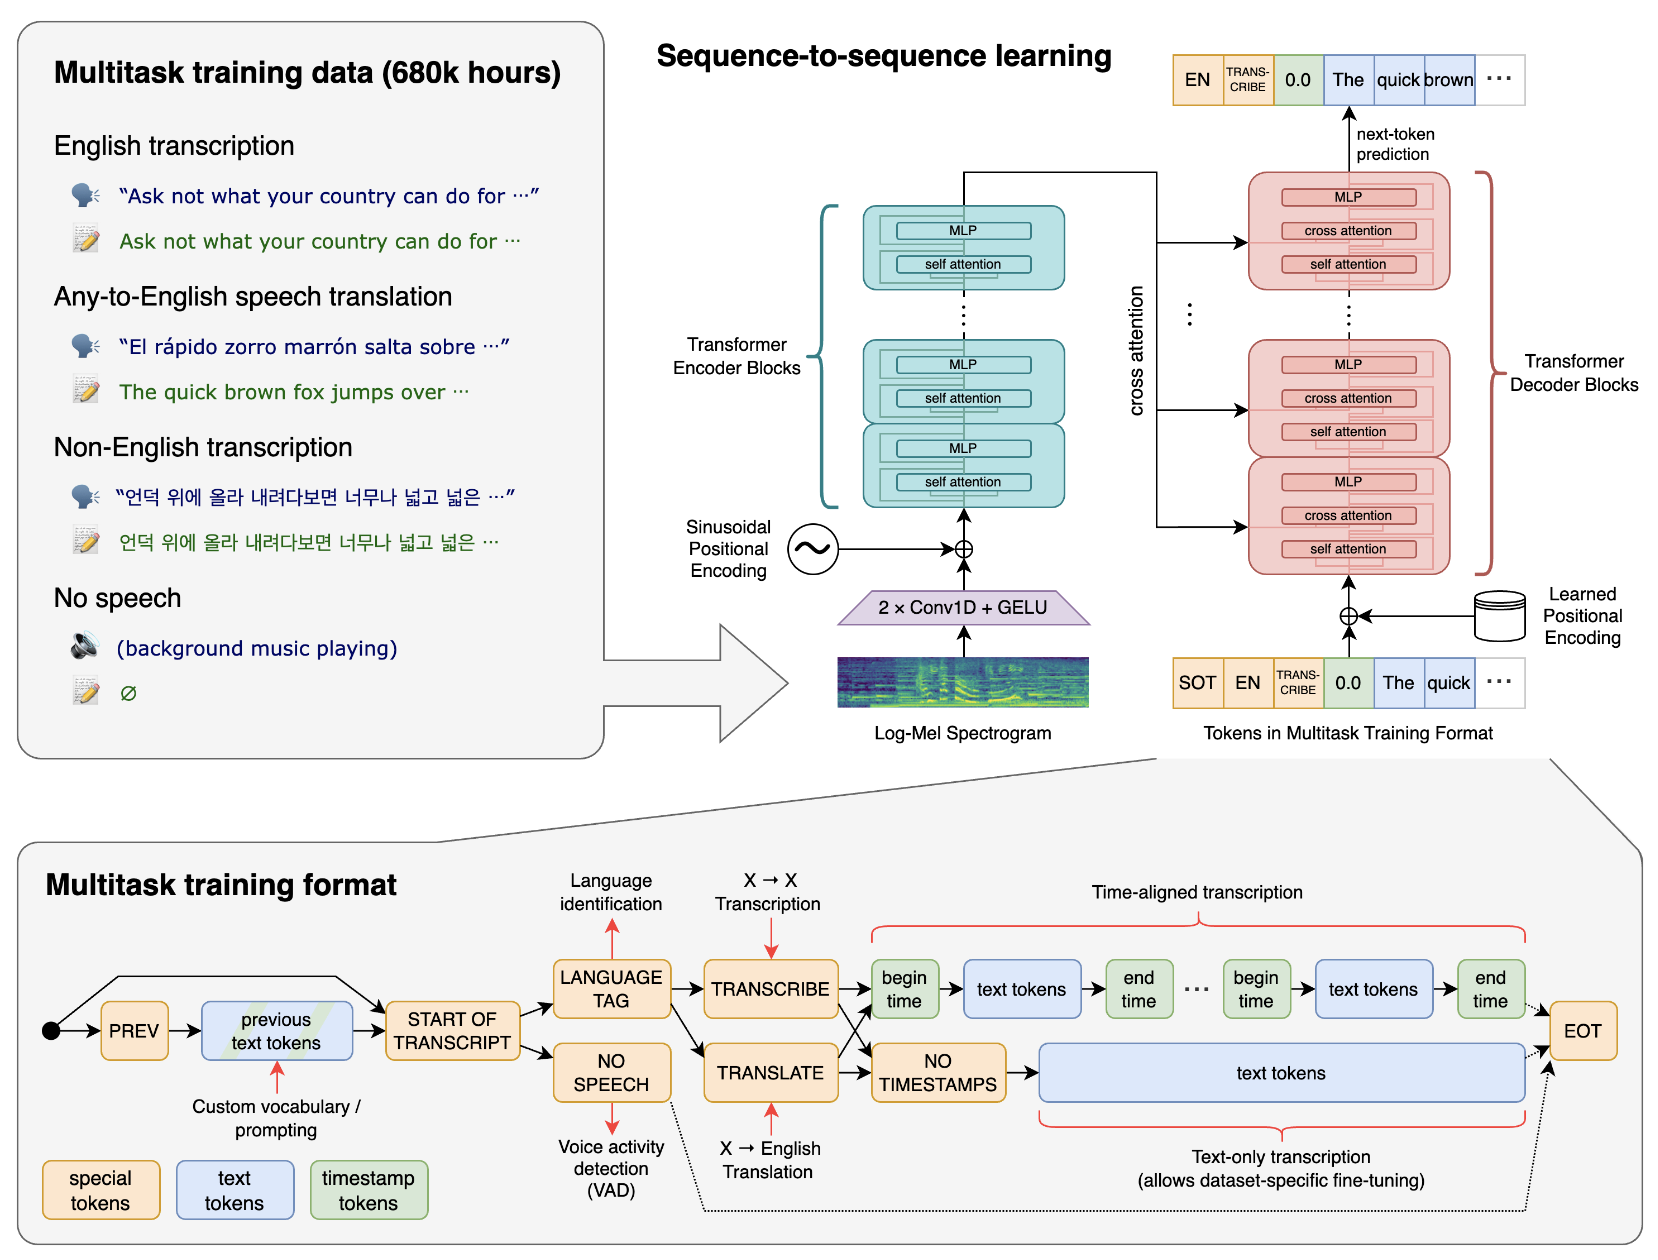
\includegraphics[width=1\linewidth]{img//intro/openai-whisper-architecture.png}
\captionof{figure}{OpenAI Whisper Architecture (source: Whisper GitHub repo)}

\section{What we Learned}

In this lesson, we learned how to:

\begin{itemize}
    \item Differentiate between Artificial Intelligence, Machine Learning, and Deep Learning to ensure that we are using the correct language to understand and communicate about our models
    \item Recognize opportunities for and limitations of Deep Learning, and choose the right model for our needs by understanding how experts think about deep learning and when to use Deep Learning
    \item Contextualize our learning by looking at the origin and history of Deep Learning
    \item Describe the value of Deep Learning by seeing applications for the models
\end{itemize}
All of these skills provide an intellectual foundation for us to learn about Deep Learning and enable us to put the things we learn into a larger framework.

\section{Glossary}

For your reference, here are all the new terms we introduced in this lesson:

\begin{itemize}
    \item \textbf{Artificial Intelligence} is the overarching field and includes algorithms like Local Search and Logic Programming
    \item \textbf{Machine Learning} is a part of Artificial Intelligence and includes models like Logistic Regression and Decision Trees
    \item \textbf{Deep Learning} is a subfield of Machine Learning that consists of various neural network models.
\end{itemize}
